\caption{step 2}
\label{Figure::inner_decision_step2}
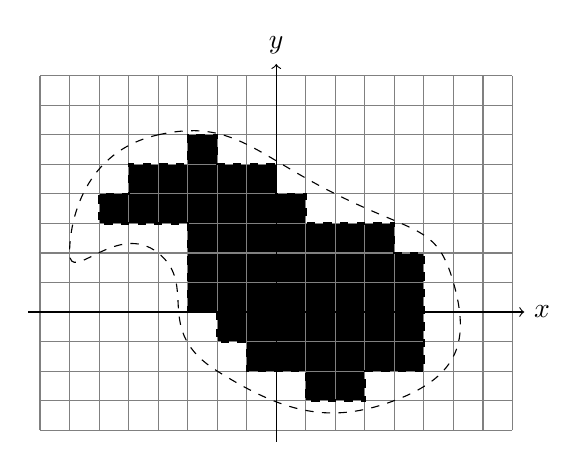
\begin{tikzpicture}[scale=0.75]

    % Define parameters
    \def\xmin{-4}
    \def\xmax{4}
    \def\ymin{-2}
    \def\ymax{4}

    % level 1
    \fill[\stepOneColor] (-1, 0) rectangle (0, 2);
    
    \fill[\stepOneColor] (0, -1) rectangle (2, 1);
    % level 2

    \fill[\stepTwoColor] (-1,-0.5) rectangle (-0.5,0);
    \fill[\stepTwoColor] (-0.5,-1) rectangle (0,0);
    \fill[\stepTwoColor] (0.5,-1.5) rectangle (1.5,-1);
    \fill[\stepTwoColor] (2,-1) rectangle (2.5,1);
    \fill[\stepTwoColor] (0,1) rectangle (2,1.5);
    \fill[\stepTwoColor] (0,1.5) rectangle (0.5,2);
    \fill[\stepTwoColor] (-1.5,0) rectangle (-1,3);
    \fill[\stepTwoColor] (-1,2) rectangle (0,2.5);
    \fill[\stepTwoColor] (-2.5,1.5) rectangle (-1.5,2.5);
    \fill[\stepTwoColor] (-3,1.5) rectangle (-2.5,2);

    \draw[step=.5,gray,thin] (\xmin,\ymin) grid (\xmax,\ymax);

    % Axes
    \draw[->] (\xmin-0.2, 0) -- (\xmax+0.2, 0) node[right] {$x$};
    \draw[->] (0, \ymin-0.2) -- (0, \ymax+0.2) node[above] {$y$};
    
    \draw[dashed] plot [smooth cycle, tension=1] coordinates {(-3.5,1) (-2,3) (1,2) (3,0.5) (2,-1.5) (-1,-1)  (-2,1) };
    \draw[dashed, thick, black](-1,0) -- (-1,-0.5) -- (-0.5, -0.5) -- (-0.5, -1) -- (0.5, -1) -- (0.5, -1.5) -- (1.5,-1.5) -- (1.5,-1) -- (1.5, -1) -- (2.5, -1) -- (2.5, 1) -- (2, 1) -- (2, 1.5) -- (0.5, 1.5) -- (0.5, 1.5) -- (0.5,2)--(0, 2) -- (0, 2.5) -- (-1, 2.5) -- (-1, 3) -- (-1.5, 3) -- (-1.5, 2.5) -- (-2.5, 2.5) -- (-2.5, 2) -- (-3, 2) -- (-3,1.5) -- (-1.5, 1.5) -- (-1.5,0) -- (-1,0);

\end{tikzpicture}
